% Copyright (c) 2017 Alexander Bluhm <bluhm@openbsd.org>
%
% Permission to use, copy, modify, and distribute this software for any
% purpose with or without fee is hereby granted, provided that the above
% copyright notice and this permission notice appear in all copies.
%
% THE SOFTWARE IS PROVIDED "AS IS" AND THE AUTHOR DISCLAIMS ALL WARRANTIES
% WITH REGARD TO THIS SOFTWARE INCLUDING ALL IMPLIED WARRANTIES OF
% MERCHANTABILITY AND FITNESS. IN NO EVENT SHALL THE AUTHOR BE LIABLE FOR
% ANY SPECIAL, DIRECT, INDIRECT, OR CONSEQUENTIAL DAMAGES OR ANY DAMAGES
% WHATSOEVER RESULTING FROM LOSS OF USE, DATA OR PROFITS, WHETHER IN AN
% ACTION OF CONTRACT, NEGLIGENCE OR OTHER TORTIOUS ACTION, ARISING OUT OF
% OR IN CONNECTION WITH THE USE OR PERFORMANCE OF THIS SOFTWARE.

\documentclass[14pt,aspectratio=169]{beamer}
%\usepackage[nomixage,puffy]{genuaslides}
\usetheme{Frankfurt}
\usepackage{tikz}
\usetikzlibrary{shapes.geometric}
\usepackage{adjustbox}
\usepackage{graphicx}
\graphicspath{{./gnuplot/}}

\author{Alexander Bluhm}
\title{Measuring Performance on OpenBSD}
\institute{bluhm@openbsd.org}
\date{BSDCan, May 2019}

\begin{document}

\begin{frame}
\titlepage
\end{frame}

\begin{frame}{Perfomance Measurement}
\setcounter{tocdepth}{1}
\tableofcontents
\end{frame}

\section{What did exist before?}

\begin{frame}{Agenda}
\setcounter{tocdepth}{1}
\tableofcontents[currentsection]
\end{frame}

\subsection{genua Firewall Testbed HPF}
\begin{frame}{genua Firewall Testbed HPF}
Numbers for
\begin{itemize}
    \item Customers
    \item Marketing
    \item Developers
    \item Hardware
    \item \dots
\end{itemize}
\end{frame}

\subsection{HPF Result}
\begin{frame}{HPF Result}
    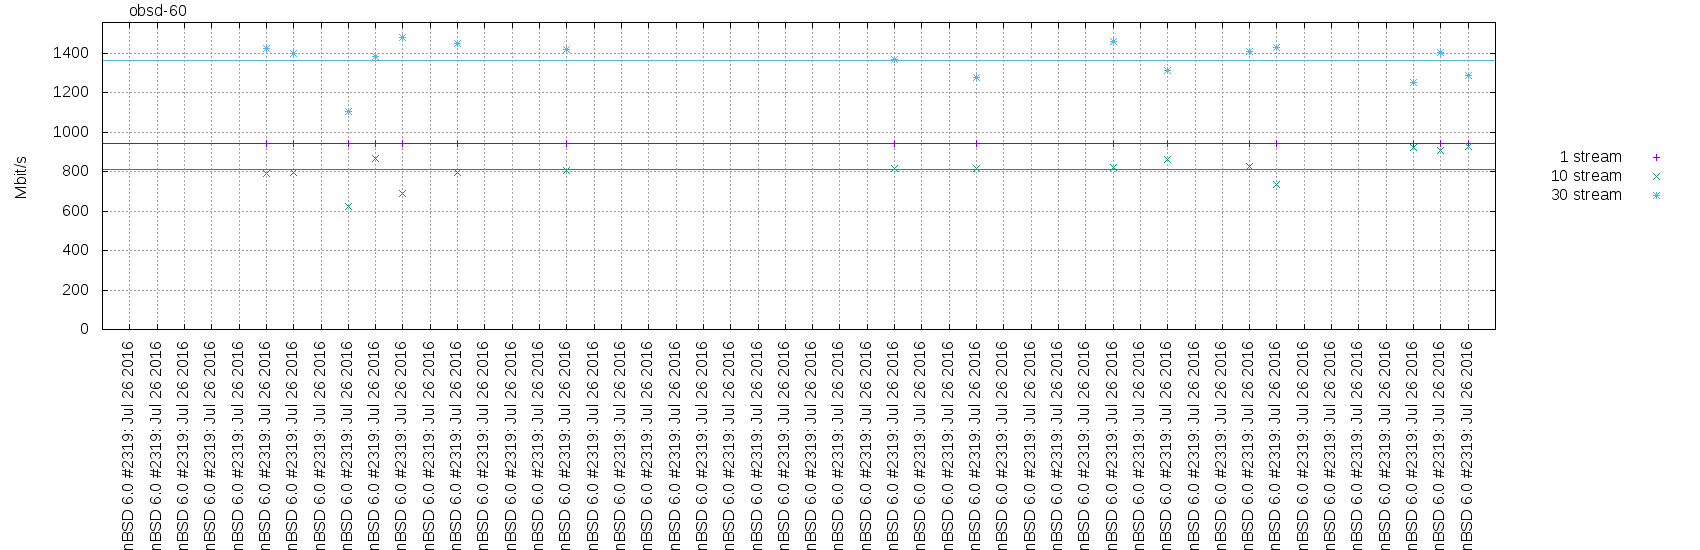
\includegraphics[width=\textwidth]{images/gs700r7_obsd_proxy_tcp.png}
\end{frame}

\subsection{Multi User, Multi Purpose Hardware Setup}
\begin{frame}{Multi User, Multi Purpose Hardware Setup}
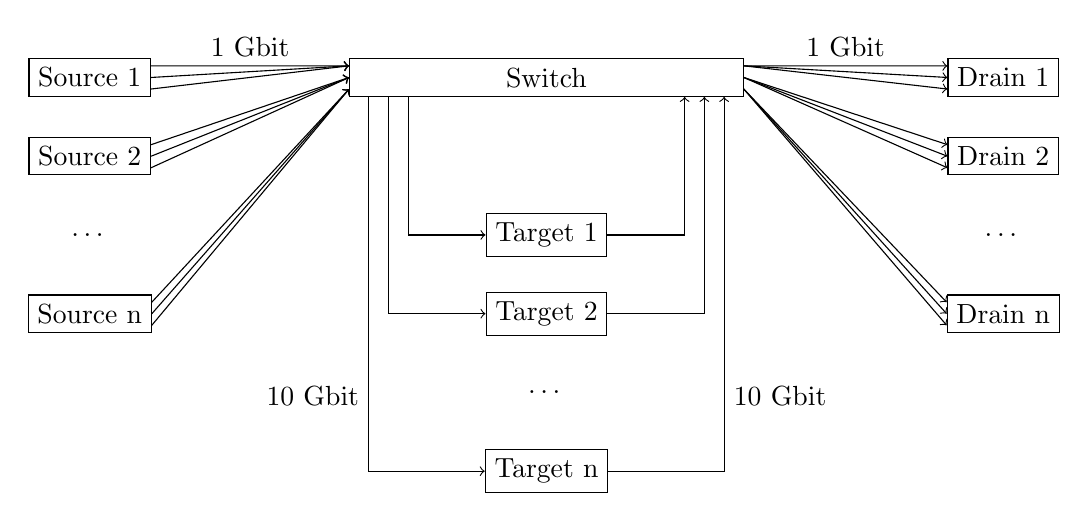
\begin{tikzpicture}
    \path (-5.8, 0) node [draw] (s1) {Source 1};
    \path (-5.8,-1) node [draw] (s2) {Source 2};
    \path (-5.8,-2) node             {\dots};
    \path (-5.8,-3) node [draw] (s3) {Source n};
    \path (s1.north east) -- (s1.south east)
     node (s11) [pos=0.2] {} node (s12) [pos=0.5] {} node (s13) [pos=0.8] {};
    \path (s2.north east) -- (s2.south east)
     node (s21) [pos=0.2] {} node (s22) [pos=0.5] {} node (s23) [pos=0.8] {};
    \path (s3.north east) -- (s3.south east)
     node (s31) [pos=0.2] {} node (s32) [pos=0.5] {} node (s33) [pos=0.8] {};

    \path ( 0, 0) node [draw,minimum width=5cm] (s)  {Switch};
    \path (s.north west) -- (s.south west)
     node (sw1) [pos=0.2] {} node (sw2) [pos=0.5] {} node (sw3) [pos=0.8] {};
    \path (s.north east) -- (s.south east)
     node (se1) [pos=0.2] {} node (se2) [pos=0.5] {} node (se3) [pos=0.8] {};

    \path ( 5.8, 0) node [draw] (d1) {Drain 1};
    \path ( 5.8,-1) node [draw] (d2) {Drain 2};
    \path ( 5.8,-2) node             {\dots};
    \path ( 5.8,-3) node [draw] (d3) {Drain n};
    \path (d1.north west) -- (d1.south west)
     node (d11) [pos=0.2] {} node (d12) [pos=0.5] {} node (d13) [pos=0.8] {};
    \path (d2.north west) -- (d2.south west)
     node (d21) [pos=0.2] {} node (d22) [pos=0.5] {} node (d23) [pos=0.8] {};
    \path (d3.north west) -- (d3.south west)
     node (d31) [pos=0.2] {} node (d32) [pos=0.5] {} node (d33) [pos=0.8] {};

    \draw [->] (s11.center) -- (sw1.center) node [pos=.5,above] {1 Gbit};
    \draw [->] (s12.center) -- (sw1.center);
    \draw [->] (s13.center) -- (sw1.center);
    \draw [->] (s21.center) -- (sw2.center);
    \draw [->] (s22.center) -- (sw2.center);
    \draw [->] (s23.center) -- (sw2.center);
    \draw [->] (s31.center) -- (sw3.center);
    \draw [->] (s32.center) -- (sw3.center);
    \draw [->] (s33.center) -- (sw3.center);

    \draw [<-] (d11.center) -- (se1.center) node [pos=.5,above] {1 Gbit};
    \draw [<-] (d12.center) -- (se1.center);
    \draw [<-] (d13.center) -- (se1.center);
    \draw [<-] (d21.center) -- (se2.center);
    \draw [<-] (d22.center) -- (se2.center);
    \draw [<-] (d23.center) -- (se2.center);
    \draw [<-] (d31.center) -- (se3.center);
    \draw [<-] (d32.center) -- (se3.center);
    \draw [<-] (d33.center) -- (se3.center);

    \path (0,-2) node [draw] (t1) {Target 1};
    \path (0,-3) node [draw] (t2) {Target 2};
    \path (0,-4) node             {\dots};
    \path (0,-5) node [draw] (t3) {Target n};
    \path (s.south) -- (s.south west)
     node (ssw1) [pos=.7] {} node (ssw2) [pos=.8] {} node (ssw3) [pos=.9] {};
    \draw [->] (ssw1.center) |- (t1.west);
    \draw [->] (ssw2.center) |- (t2.west);
    \draw [->] (ssw3.center) |- (t3.west) node [pos=.4,left]{10 Gbit};
    \path (s.south) -- (s.south east)
     node (sse1) [pos=.7] {} node (sse2) [pos=.8] {} node (sse3) [pos=.9] {};
    \draw [<-] (sse1.center) |- (t1.east);
    \draw [<-] (sse2.center) |- (t2.east);
    \draw [<-] (sse3.center) |- (t3.east) node [pos=.4,right]{10 Gbit};
\end{tikzpicture}
\end{frame}

\subsection{Unsuitable HPF}
\begin{frame}{Unsuitable HPF}
\begin{itemize}
    \item too many requirements
    \item too much complexity
    \item not enough flexibility
\end{itemize}
\end{frame}

\subsection{Performance Hardware Design}
\begin{frame}{Performance Hardware Design}
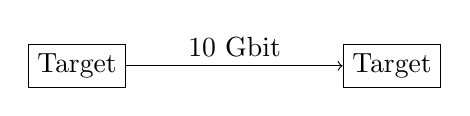
\begin{tikzpicture}
    \path (  0,   0) node [draw] (local) {Target};
    \path (  4,   0) node [draw] (remote) {Target};
    \draw [->] (local) -- (remote) node [midway,above] {10 Gbit};
\end{tikzpicture}
\end{frame}

\subsection{Existing Regression Tests}
\begin{frame}{Existing Regression Tests}
\begin{itemize}
    \item daily test runs
    \item using /usr/src/regress
    \item multi architecture
    \item history of pass and fail
    \item useful information
    \item web access \url{http://bluhm.genua.de/}
\end{itemize}
\end{frame}

\subsection{All Regression Tests}
\begin{frame}{All Regression Tests}
    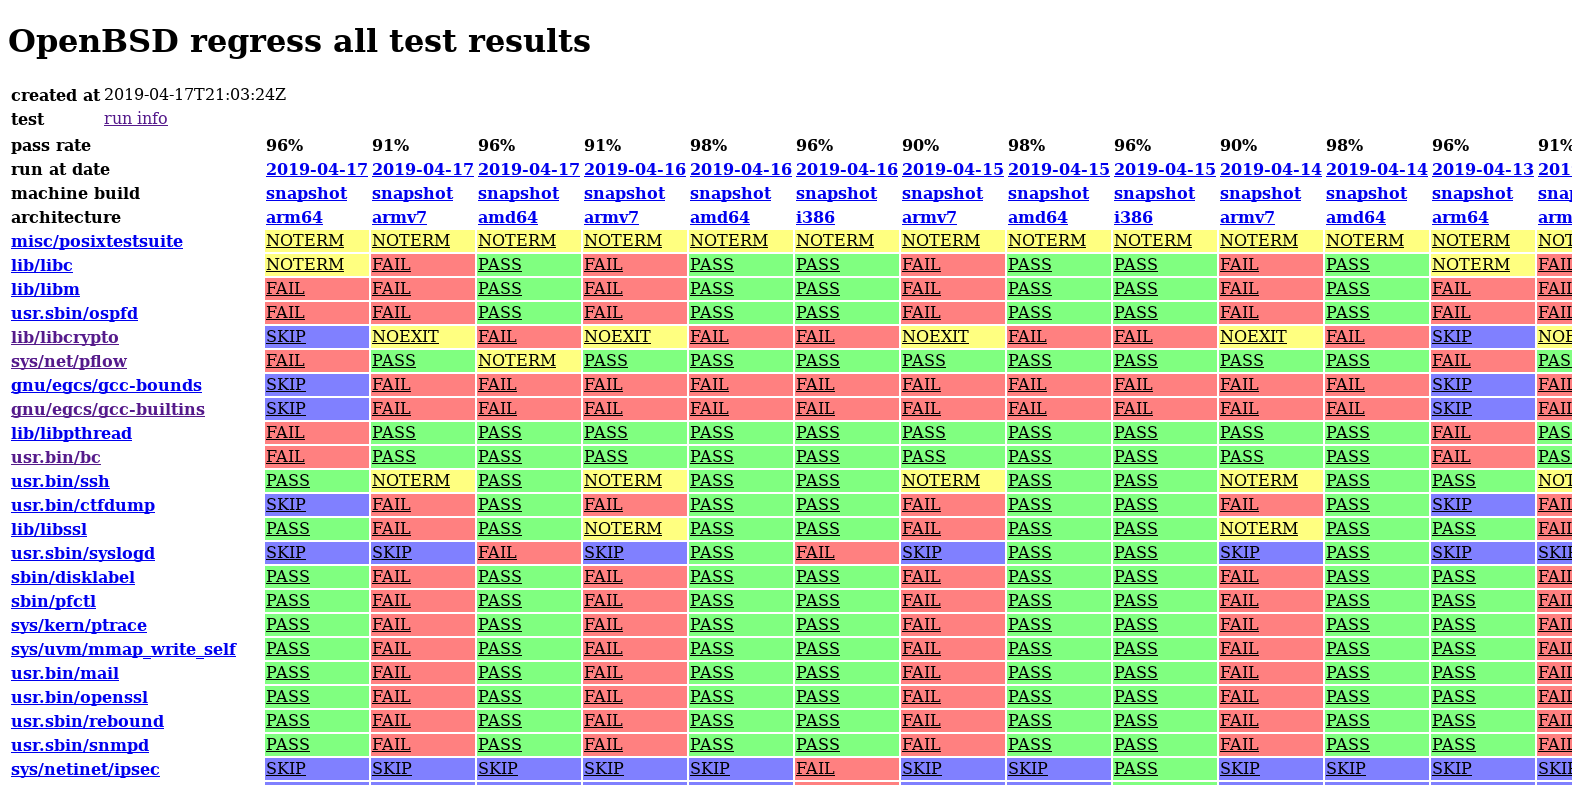
\includegraphics[width=\textwidth,trim=0 4cm 0 0,clip]
	{images/screenshot_regress_all.png}
\end{frame}

\subsection{Regression Tests with Links}
\begin{frame}{Regression Tests with Links}
\begin{tikzpicture}
    \path (0,0) node [anchor=north west]
	{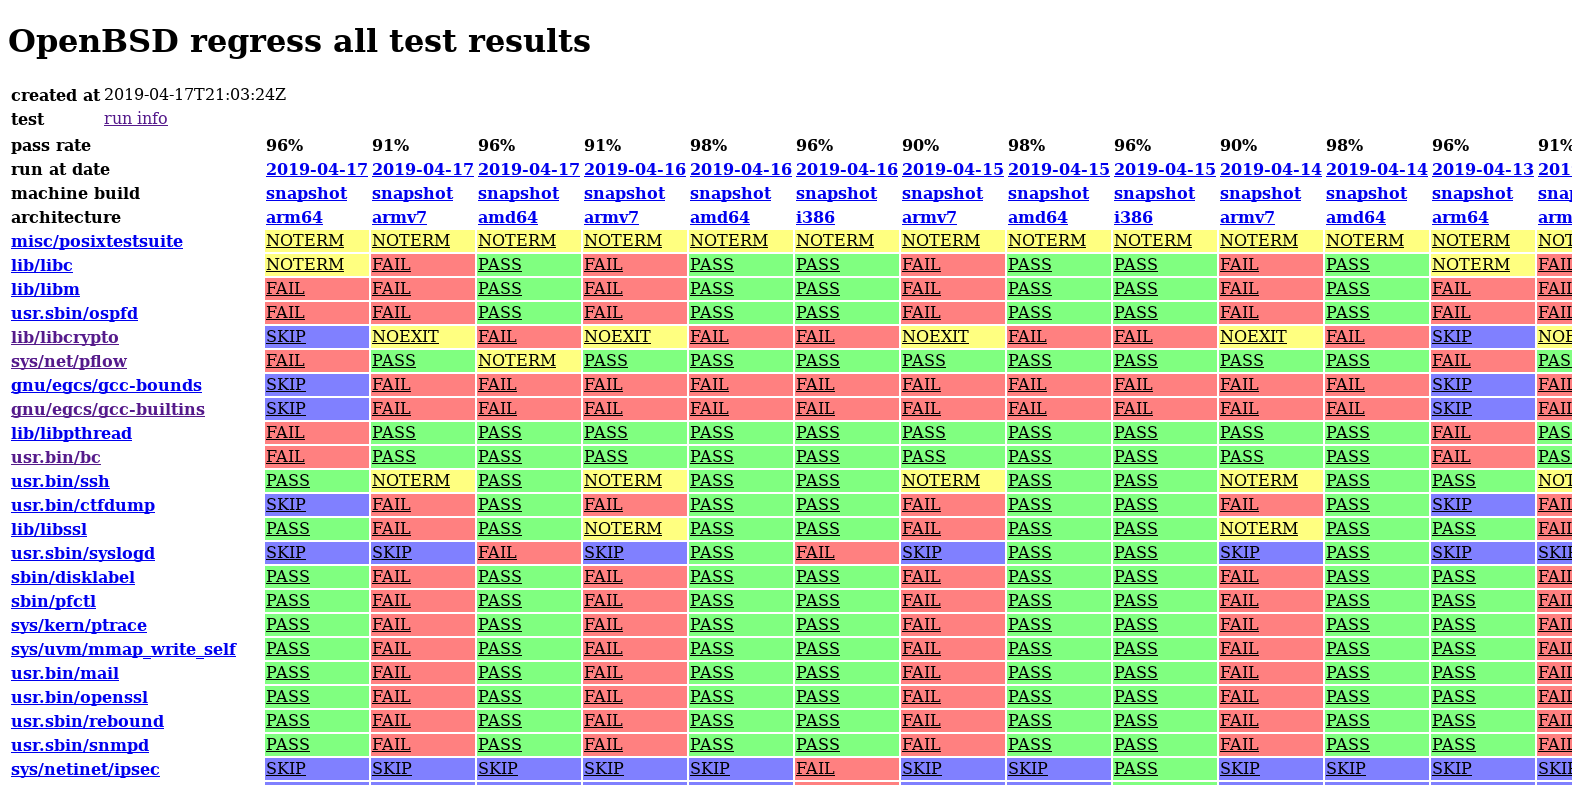
\includegraphics[width=10cm,trim=0 7cm 37cm 0,clip]
	{images/screenshot_regress_all.png}};
    \path (-1.3,-.7) node (n1) [red] {run history};
    \path (1.2,-1.1) node (e1) [ellipse,minimum width=1cm,draw,red,thick] {};
    \draw [draw,red,thick,->] (n1) -- (e1);
    \path (-1.5,-2.1) node (n2) [red] {cvs web};
    \path (.5,-2.35) node (e2) [ellipse,minimum width=1cm,draw,red,thick] {};
    \draw [draw,red,thick,->] (n2) -- (e2);
    \path (-1.5,-3.5) node (n3) [red,align=center] {colored\\status};
    \path (3,-3.8) node (e3) [ellipse,minimum width=2cm,draw,red,thick] {};
    \draw [draw,red,thick,->] (n3) -- (e3);
    \path (-1.5,-5.3) node (n4) [red] {test output};
    \path (3.2,-4.8) node (e4) [ellipse,minimum width=1cm,draw,red,thick] {};
    \draw [draw,red,thick,->] (n4) -- (e4);
    \path (6.5,0) node (n5) [red,align=center] {setup logs\\obj download};
    \path (4.2,-1.45) node (e5) [ellipse,minimum width=1cm,draw,red,thick] {};
    \draw [draw,red,thick,->] (n5) -- (e5);
    \path (9,0) node (n6) [red,align=center] {tested\\version};
    \path (6.5,-1.7) node (e6) [ellipse,minimum width=1cm,draw,red,thick] {};
    \draw [draw,red,thick,->] (n6) -- (e6);
\end{tikzpicture}
\end{frame}

\subsection{Regression History for i386}
\begin{frame}{Regression History for i386}
\begin{tikzpicture}
    \path (0,0) node [anchor=north west]
	{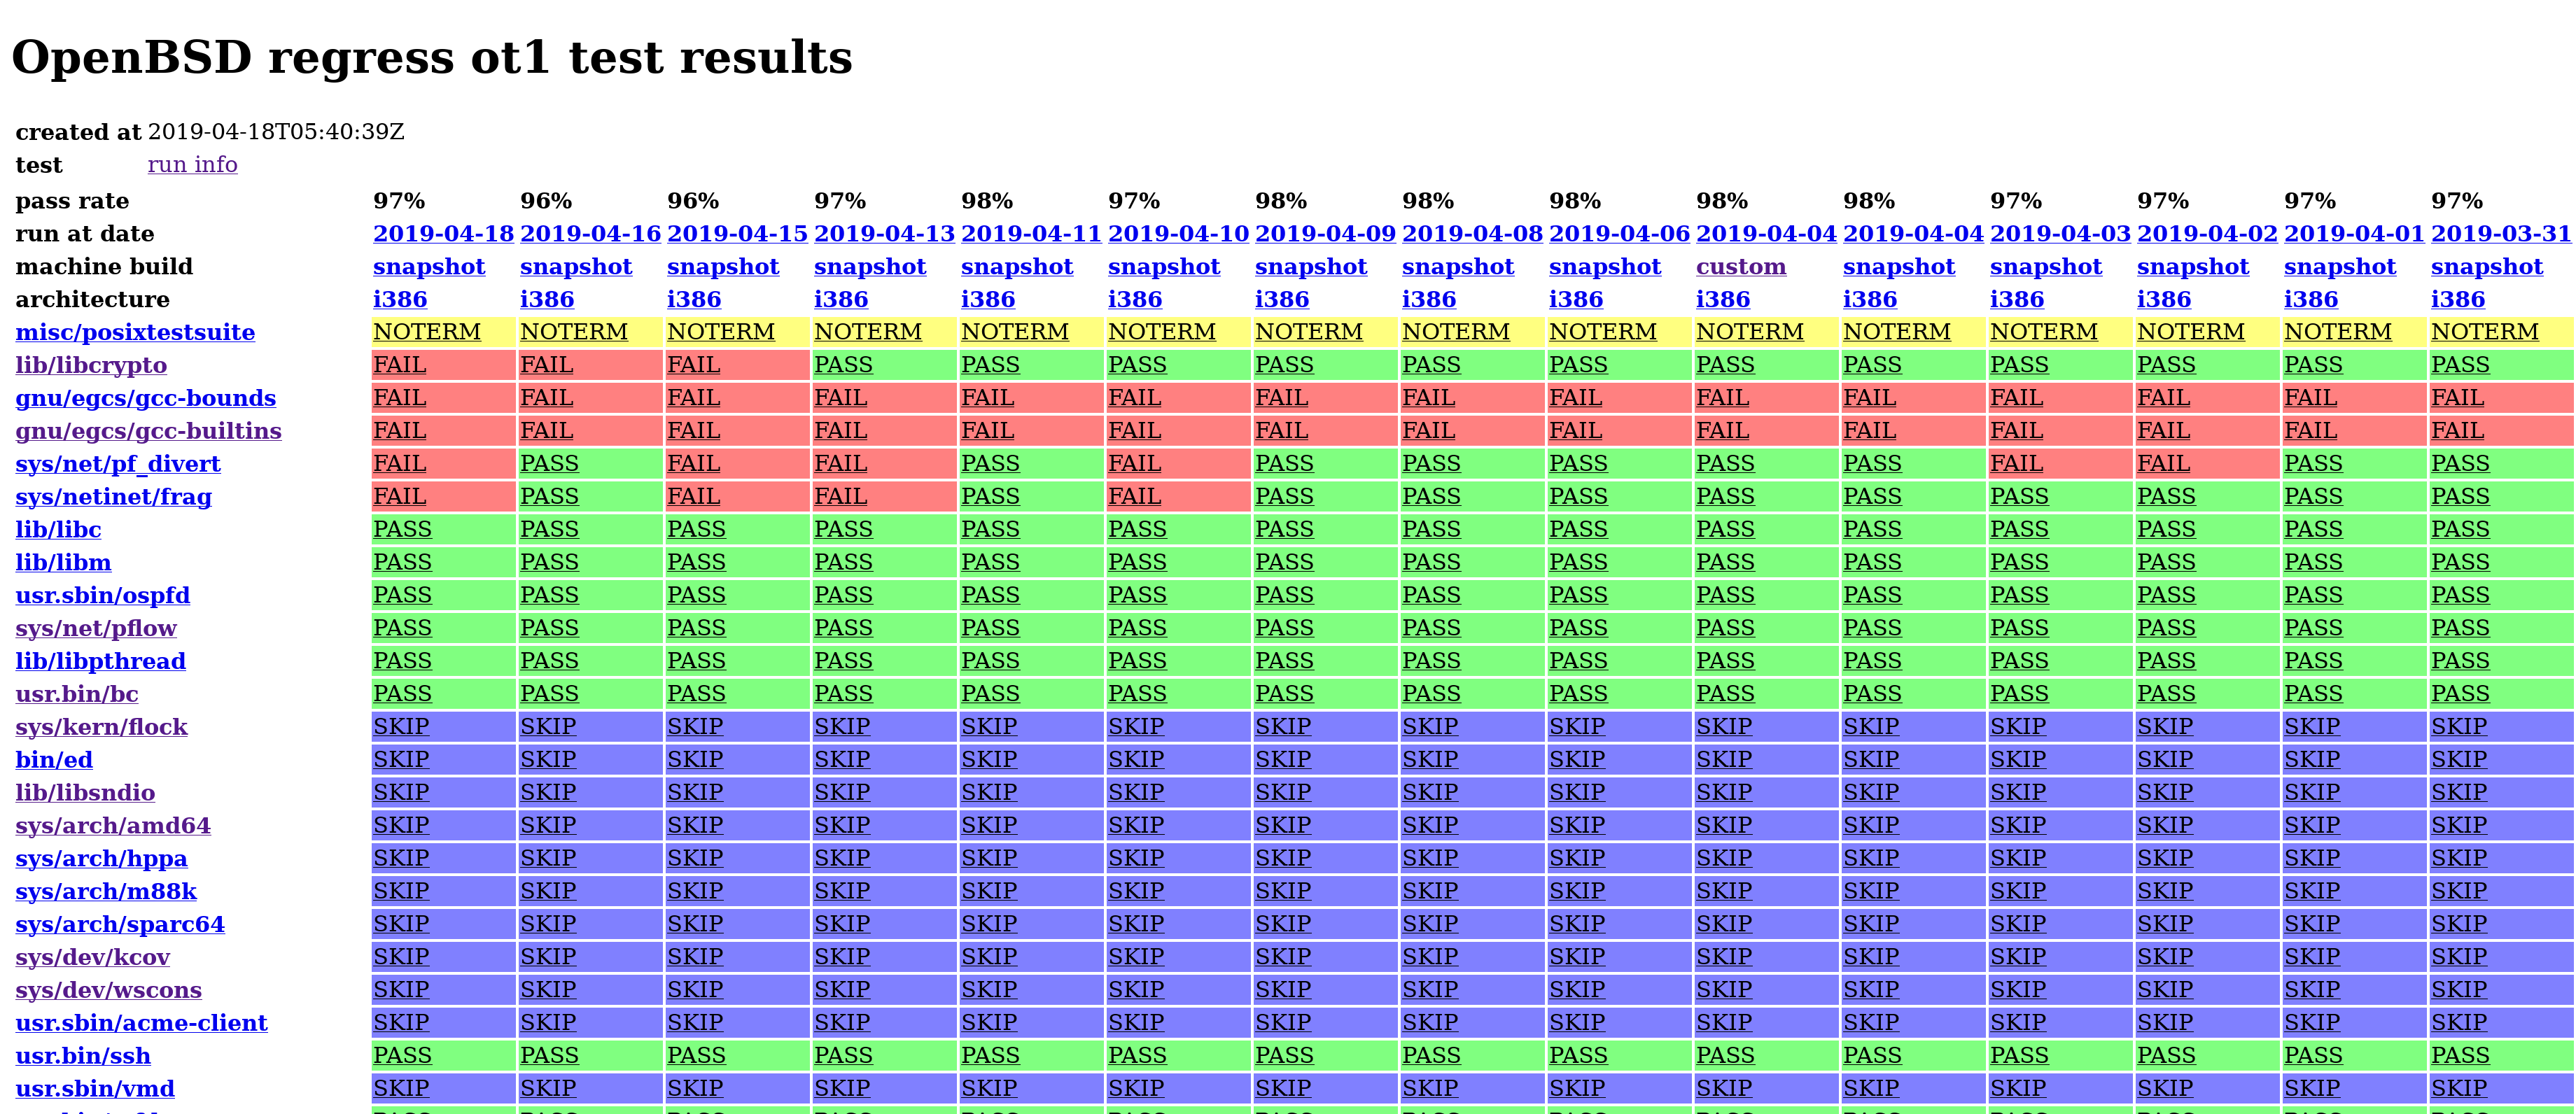
\includegraphics[width=10cm,trim=0 7cm 37cm 0,clip]
	{images/screenshot_regress_ot1.png}};
    \draw [draw,red,thick,->] (1.6,0) -- (10.8,0)
	node [midway,above] {history};
    \draw [draw,red,thick,<-] (-.2,-1.5) -- (-.2,-5.8)
	node [midway,left] {severity};
\end{tikzpicture}
\end{frame}

\subsection{Regression Test Hardware}
\begin{frame}{Regression Test Hardware}
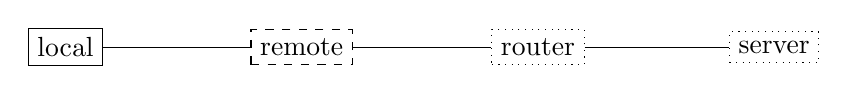
\begin{tikzpicture}
    \path (  0,   0) node [draw] (local) {local};
    \path (  3,   0) node [draw,dashed] (remote) {remote};
    \path (  6,   0) node [draw,dotted] (router) {router};
    \path (  9,   0) node [draw,dotted] (server) {server};
    \draw (local) -- (remote);
    \draw (remote) -- (router);
    \draw (router) -- (server);
\end{tikzpicture}
\end{frame}

\subsection{Regression Master}
\begin{frame}{Regression Master}
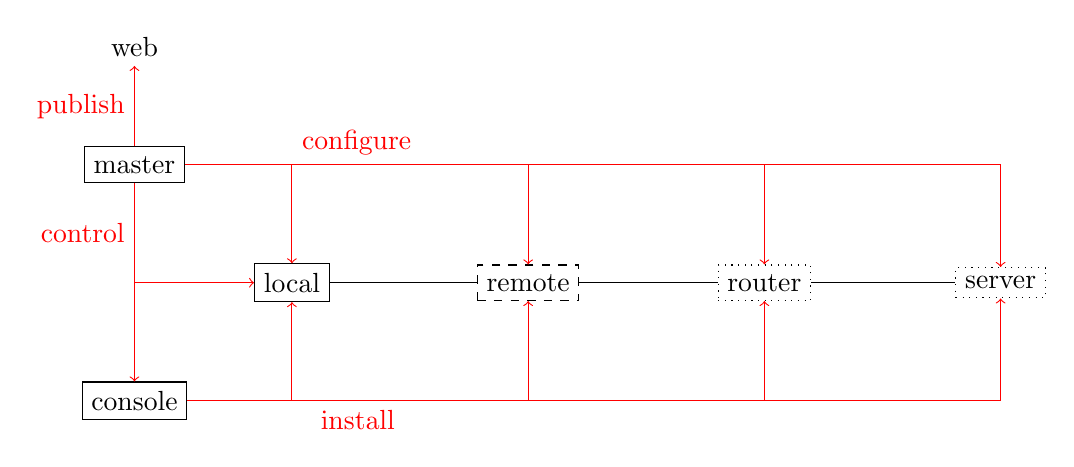
\begin{tikzpicture}
    \path ( -2,   3) node (web) {web};
    \path ( -2, 1.5) node [draw] (master) {master};
    \path (  0,   0) node [draw] (local) {local};
    \path (  3,   0) node [draw,dashed] (remote) {remote};
    \path (  6,   0) node [draw,dotted] (router) {router};
    \path (  9,   0) node [draw,dotted] (server) {server};
    \path ( -2,-1.5) node [draw] (console) {console};
    \draw (local) -- (remote);
    \draw (remote) -- (router);
    \draw (router) -- (server);
    \draw [->,red] (master) -- (web) node [midway,left] {publish};
    \draw [->,red] (master) -- (console);
    \draw [->,red] (master) |- (local) node [near start,left] {control};
    \draw [->,red] (master) -| (local);
    \draw [->,red] (master) -| (remote) node [near start,above] {configure};
    \draw [->,red] (master) -| (router);
    \draw [->,red] (master) -| (server);
    \draw [->,red] (console) -| (local);
    \draw [->,red] (console) -| (remote) node [near start,below] {install};
    \draw [->,red] (console) -| (router);
    \draw [->,red] (console) -| (server);
\end{tikzpicture}
\end{frame}

\section{How does it work?}

\begin{frame}{Agenda}
\setcounter{tocdepth}{1}
\tableofcontents[currentsection]
\end{frame}

\subsection{Performance Goals}
\begin{frame}{Performance Goals}
\begin{itemize}
    \item history
    \item reproducable
    \item details available
    \item drill down
    \item automatic
\end{itemize}
\end{frame}

\subsection{Performance History}
\begin{frame}{Performance History}
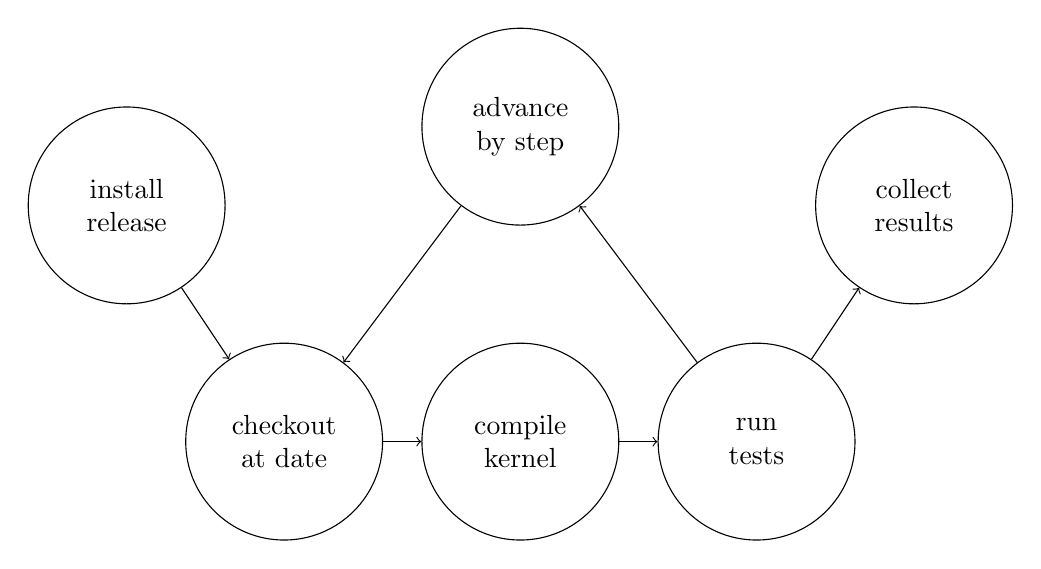
\begin{tikzpicture}
    \path ( 1, 1) node [draw,circle,align=center,minimum width=2.5cm]
	(release) {install\\release};
    \path ( 3,-2) node [draw,circle,align=center,minimum width=2.5cm]
	(checkout) {checkout\\at date};
    \path ( 6,-2) node [draw,circle,align=center,minimum width=2.5cm]
	(kernel) {compile\\kernel};
    \path ( 9,-2) node [draw,circle,align=center,minimum width=2.5cm]
	(test) {run\\tests};
    \path ( 6, 2) node [draw,circle,align=center,minimum width=2.5cm]
	(step) {advance\\by step};
    \path (11, 1) node [draw,circle,align=center,minimum width=2.5cm]
	(result) {collect\\results};
    \draw [->] (release) -- (checkout);
    \draw [->] (checkout) -- (kernel);
    \draw [->] (kernel) -- (test);
    \draw [->] (test) -- (result);
    \draw [->] (test) -- (step);
    \draw [->] (step) -- (checkout);
\end{tikzpicture}
\end{frame}

\subsection{Weekly from 6.2 to 6.3}
\begin{frame}{Weekly from 6.2 to 6.3}
    \begin{adjustbox}{totalheight=\textheight-2\baselineskip}
	\input{gnuplot/2019-02-04T15-10-35Z-tcp.tex}
    \end{adjustbox}
\end{frame}

\subsection{Build Quirks}
\begin{frame}{Build Quirks}
\begin{tikzpicture}
    \path ( 3,-2) node [draw,circle,align=center,minimum width=2.5cm]
	(checkout) {checkout\\at date};
    \path ( 6,-2) node [draw,circle,align=center,minimum width=2.5cm]
	(kernel) {compile\\kernel};
    \path ( 9,-2) node [draw,circle,align=center,minimum width=2.5cm]
	(test) {run\\tests};
    \path ( 9, 2) node [draw,circle,align=center,minimum width=2.5cm]
	(step) {advance\\by step};
    \path ( 6, 2) node [draw,circle,align=center,minimum width=2.5cm]
	(userland) {checkout\\userland};
    \path ( 3, 2) node [draw,circle,align=center,minimum width=2.5cm]
	(toolchain) {build\\toolchain};
    \draw [->] (release) -- (checkout);
    \draw [->] (checkout) -- (kernel);
    \draw [->] (kernel) -- (test);
    \draw [->] (test) -- (result);
    \draw [->] (test) -- (step);
    \draw [->] (step) -- (checkout);
    \draw [->] (step) -- (userland);
    \draw [->] (userland) -- (toolchain);
    \draw [->] (toolchain) -- (checkout);
\end{tikzpicture}
\end{frame}

\subsection{Quirks from 6.2 to 6.3}
\begin{frame}{Quirks from 6.2 to 6.3}
\begin{tabular}{cl}
    A & OpenBSD/amd64 6.2 release\\
    B & fix cvs vendor branch checkout\\
    C & clang update LLVM to 5.0.0\\
    D & pfctl pf packet rate matching\\
    E & move kernel source file dwiic.c\\
    F & pfctl pf divert type\\
    G & sysctl struct vfsconf\\
    H & clang update LLVM to 5.0.1\\
    I & pfctl pf syncookies\\
    J & OpenBSD/amd64 6.3 release\\
\end{tabular}
\end{frame}

\subsection{Performance Hardware Future}
\begin{frame}{Performance Hardware Future}
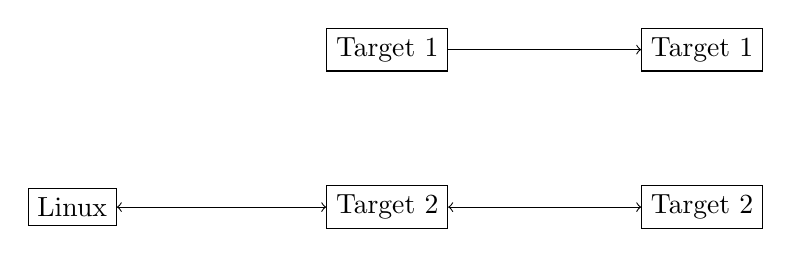
\begin{tikzpicture}
    \path (  0,   0) node [draw] (local1) {Target 1};
    \path (  4,   0) node [draw] (remote1) {Target 1};
    \draw [->] (local1) -- (remote1);
    \path (  0,  -2) node [draw] (local2) {Target 2};
    \path (  4,  -2) node [draw] (remote2) {Target 2};
    \draw [<->] (local2) -- (remote2);
    \path ( -4,  -2) node [draw] (linux) {Linux};
    \draw [<->] (linux) -- (local2);
\end{tikzpicture}
\end{frame}

\subsection{Performance Master}
\begin{frame}{Performance Master}
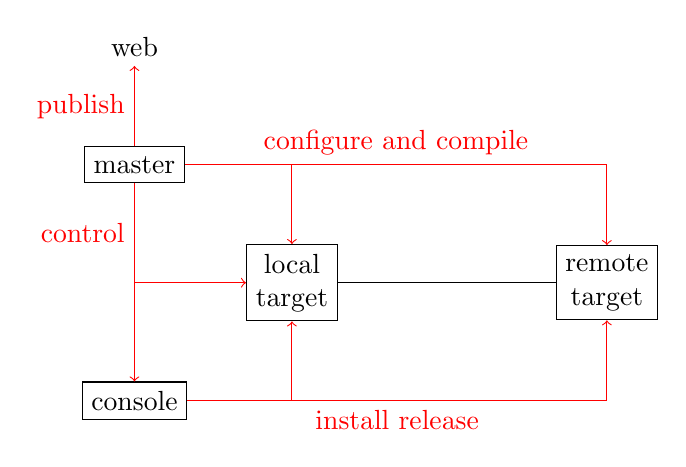
\begin{tikzpicture}
    \path ( -2,   3) node (web) {web};
    \path ( -2, 1.5) node [draw] (master) {master};
    \path ( -2,-1.5) node [draw] (console) {console};
    \path (  0,   0) node [draw,align=center] (local) {local\\target};
    \path (  4,   0) node [draw,align=center] (remote) {remote\\target};
    \draw (local) -- (remote);
    \draw [->,red] (master) -- (web) node [midway,left] {publish};
    \draw [->,red] (master) -- (console);
    \draw [->,red] (master) |- (local) node [near start,left] {control};
    \draw [->,red] (master) -| (local);
    \draw [->,red] (master) -| (remote)
	node [near start,above] {configure and compile};
    \draw [->,red] (console) -| (local);
    \draw [->,red] (console) -| (remote)
	node [near start,below] {install release};
\end{tikzpicture}
\end{frame}

\section{What are the findings?}

\begin{frame}{Agenda}
\setcounter{tocdepth}{1}
\tableofcontents[currentsection]
\end{frame}

\subsection{Reproduce and Reboot}
\begin{frame}{Reproduce and Reboot}
\begin{tikzpicture}
    \path ( 6,-2) node [draw,circle,align=center,minimum width=2.5cm]
	(kernel) {compile\\kernel};
    \path ( 9,-2) node [draw,circle,align=center,minimum width=2.5cm]
	(test) {run\\tests};
    \path (11,-4) node [draw,circle,align=center,minimum width=2.5cm]
	(keep) {run\\again};
    \path (14,-4) node [draw,circle,align=center,minimum width=2.5cm]
	(reboot) {reboot\\machine};
    \path (17,-4) node [draw,circle,align=center,minimum width=2.5cm]
	(reorder) {relink\\kernel};
    \draw [->] (checkout.east) -- (kernel);
    \draw [->] (kernel) -- (test);
    \draw [->] (test) -- (result);
    \draw [->] (test) -- (step);
    \draw [->] (test) -| (keep);
    \draw [->] (test) -| (reboot);
    \draw [->] (test) -| (reorder);
    \draw [->] (reorder) -- (reboot);
    \draw [->] (reboot) -- (keep);
    \draw [->] (keep) -| (test);
\end{tikzpicture}
\end{frame}

\subsection{5 Days, 10 Tests, Keep Machine Running}
\begin{frame}{5 Days, 10 Tests, Keep Machine Running}
    \begin{adjustbox}{totalheight=\textheight-2\baselineskip}
	\input{gnuplot/2019-03-19T14-50-23Z-tcp_7.tex}
    \end{adjustbox}
\end{frame}

\subsection{5 Days, 10 Tests, Reboot Machine}
\begin{frame}{5 Days, 10 Tests, Reboot Machine}
    \begin{adjustbox}{totalheight=\textheight-2\baselineskip}
	\input{gnuplot/2019-03-20T00-44-00Z-tcp_7.tex}
    \end{adjustbox}
\end{frame}

\subsection{5 Days, 10 Tests, Link and Reorder Kernel}
\begin{frame}{5 Days, 10 Tests, Link and Reorder Kernel}
    \begin{adjustbox}{totalheight=\textheight-2\baselineskip}
	\input{gnuplot/2019-03-20T17-37-52Z-tcp_7.tex}
    \end{adjustbox}
\end{frame}

\section{What is the Conclusion?}

\begin{frame}{Agenda}
\setcounter{tocdepth}{1}
\tableofcontents[currentsection]
\end{frame}

\subsection{Insights}
\begin{frame}{Insights}
\begin{itemize}
    \item measuring sucks
    \item multi socket CPUs sucks
    \item reproduction is hard
    \item do not trust your numbers
    \item keep is simple stupid
\end{itemize}
\end{frame}

\subsection{Thanks}
\begin{frame}{Thanks}
\begin{itemize}
    \item Jan Klemkow for Hardware Administration
    \item Moritz Buhl for Visualization
    \item genua for Hosting and Worktime
\end{itemize}
\end{frame}

\subsection{Links}
\begin{frame}{Links}
\begin{itemize}
    \small
    \item \url{http://bluhm.genua.de/}
    \item \url{http://bluhm.genua.de/regress/results/regress.html}
    \item \url{http://bluhm.genua.de/perform/results/perform.html}
    \item \url{https://github.com/bluhm/regress-all}
    \item \url{https://github.com/younix/testmaster}
    \item \url{https://github.com/bluhm/talk-perform}
\end{itemize}
\end{frame}

\end{document}
